\newpage
\subsection{Identify subsystems}
\begin{figure}[htb!]
    \centering
    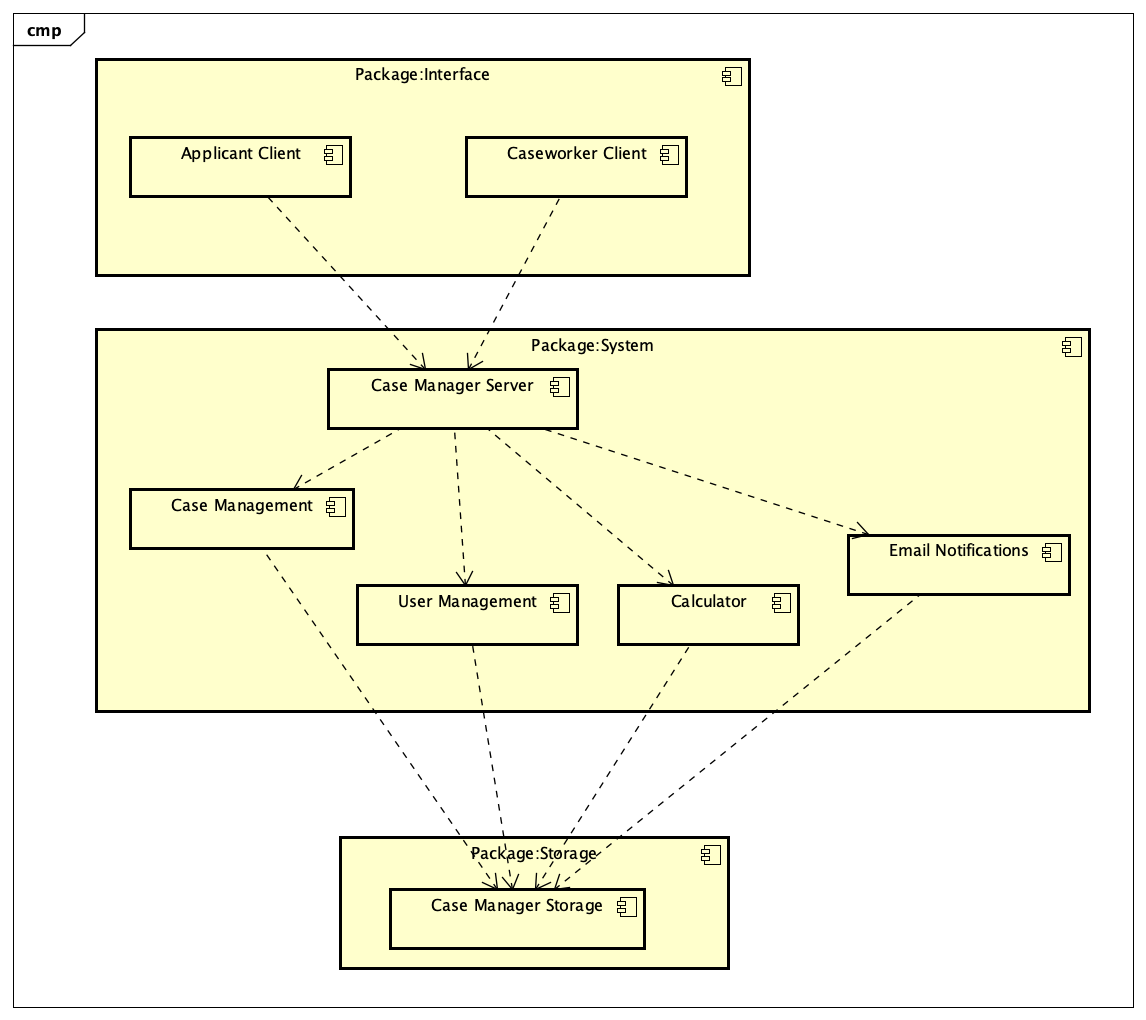
\includegraphics[width=\textwidth]{img/cmp-diagram.png}
    \caption{Component Diagram}
\end{figure}
We have identified 3 subsystems, Interface, the system and the database subsystems.
Applicant and caseworker client has high cohesion and therefore it would make sense to implement in a single client, because you have a lot of features that would be similar. Codingwise, Applicant and caseworker client are very similar, thus it's a good way of putting them as a subsystem. It is obvious that applicant and the caseworker have low coupling, or perhaps, there is no coupling at all because they don't depend in each other. \\
Similarly for the subsystem called System, we have dependency from Case Manager Server to the rest of the components, also high cohesion. 
It is a high coupling between applicant or caseworker to Case Manager Server, other than that, there are  low couplings between other components.\\
\\
We have divided this problem into 3-subsystems because  every subsystem has similar features in common. The Package Storage is made as a special subsystem in case of  unforeseen crash





  